\chapter{Testiranje performansi}

Biblioteka YAAACD izrađena je u svrhu usporedbe performansi triju vrsti
algoritama otkrivanja sudara u trodimenzionalnom prostoru.

Upoređivani algoritmi su:
\begin{enumerate}
    \item \textbf{Algoritam grube sile} - vrsta provjere u kojoj se
          provjeravaju svi primitivi dvaju učitanih objekata
    \item \textbf{Provjera korištenjem oktalnog stabla} - opisano u poglavlju \ref{chapter:octree}
    \item \textbf{Provjera korištenjem prostornog hashiranja} - opisano u poglavlju \ref{chapter:spatial}
\end{enumerate}

\section{Način testiranja}

Testiranje je izvedeno korištenjem YAAACD-GUI aplikacije, koja se brine za grafički prikaz
objekata koji se testiraju, mjerenje performansi te izvještavanje (\textit{logging}) (Slika \ref{logging}).

\begin{figure}[h!]
    \centering
    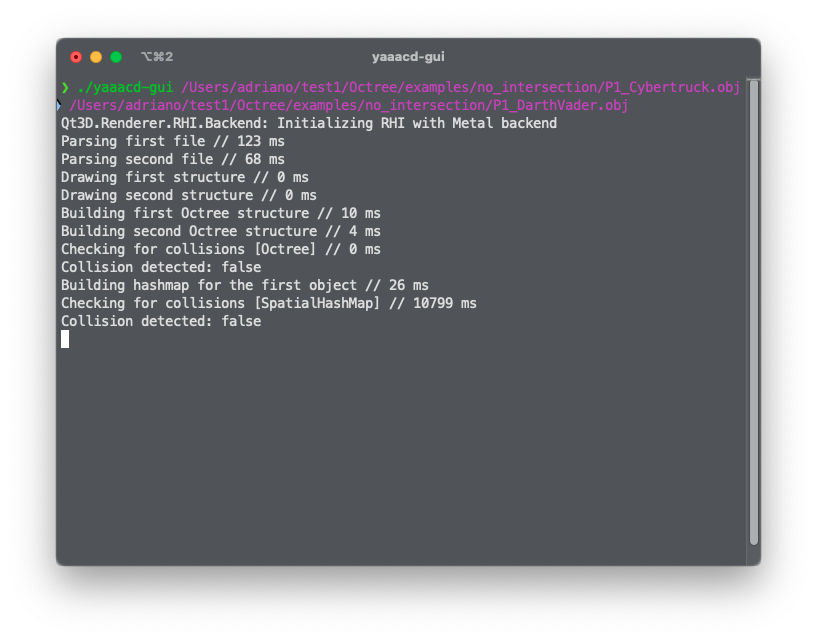
\includegraphics[width=12cm]{logs.png}
    \caption {Prikaz ispisa aplikacije YAAACD-GUI prije učitavanja.}
    \label{logging}
\end{figure}

\pagebreak
\subsection{Testno okruženje}
Sve metode korištenje pri testiranju koriste samo jednu procesorsku nit.
Testiranje je izvršeno na sustavu sa Intel Core i7 procesorom, 16 GB radne memorije
i macOS operacijskim sustavom. (Slika \ref{testbench})

\begin{figure}[h!]
    \centering
    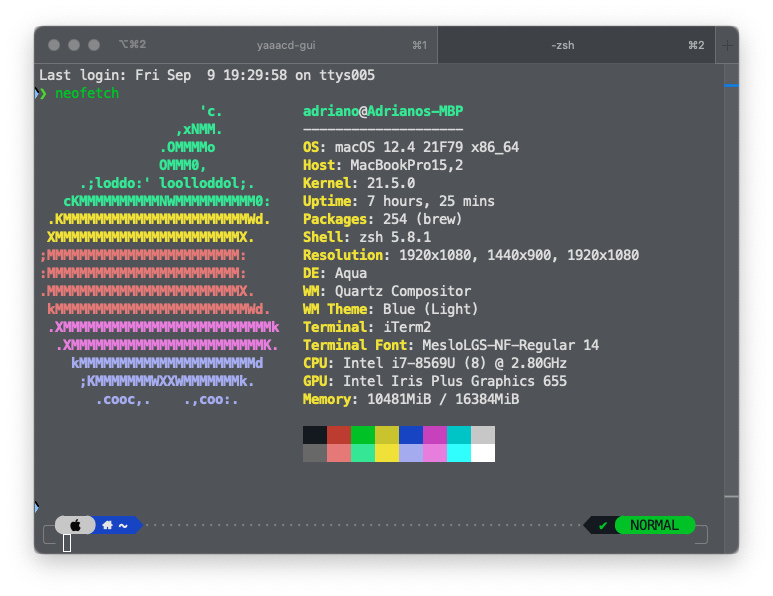
\includegraphics[width=12cm]{testbench.png}
    \caption {Prikaz informacija o testnom sustavu}
    \label{testbench}
\end{figure}

\pagebreak
\section{Rezultati testiranja}

Testiranje je izvedeno sa četiri različita 3D modela različite veličine i gustoće primitiva.
Rezultati su prikazani u tablici \ref{table:testresults}

\begin{table}[h!]
    \begin{center}
      \begin{tabular}{ | c | c | c | }
        \hline
        \textbf{Model} & \textbf{Broj točaka} & \textbf{Broj trokuta} \\
        \hline
         Spiderman (Slika \ref{model:spiderman}) & 74.999 & 149.994 \\
        \hline
         Cybertruck (Slika \ref{model:cybertruck}) & 32.273 & 63.614 \\
        \hline
         Shrek (Slika \ref{model:shrek}) & 1.274 & 2.332 \\
        \hline
         Darth Vader (Slika \ref{model:darthvader}) & 24.636 & 35.624 \\
        \hline
      \end{tabular}
    \end{center}
  \caption{Broj poligona i točaka po modelu}
  \label{table:poly}
\end{table}

\begin{figure}
    \centering
    \begin{minipage}[b]{0.4\textwidth}
        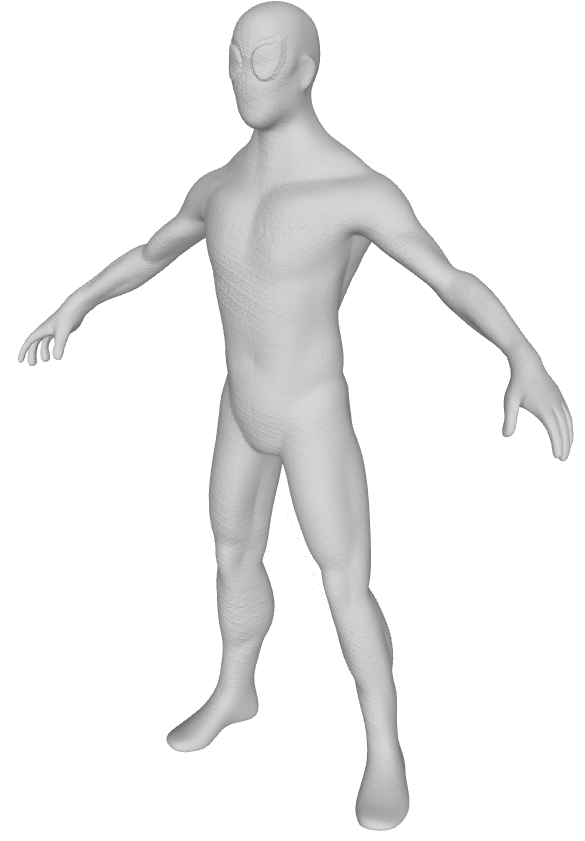
\includegraphics[width=\textwidth]{spiderman.png}
        \caption {Testni model: Spiderman}
        \label{model:spiderman}
    \end{minipage}
    \begin{minipage}[b]{0.4\textwidth}
        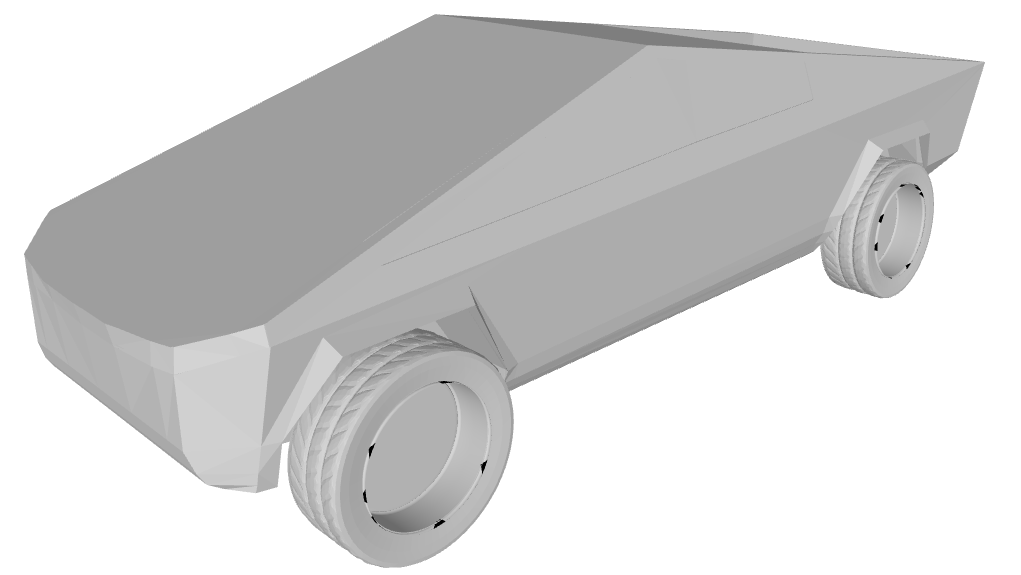
\includegraphics[width=\textwidth]{cybertruck.png}
        \caption {Testni model: Cybertruck}
        \label{model:cybertruck}
    \end{minipage}
    \begin{minipage}[b]{0.4\textwidth}
        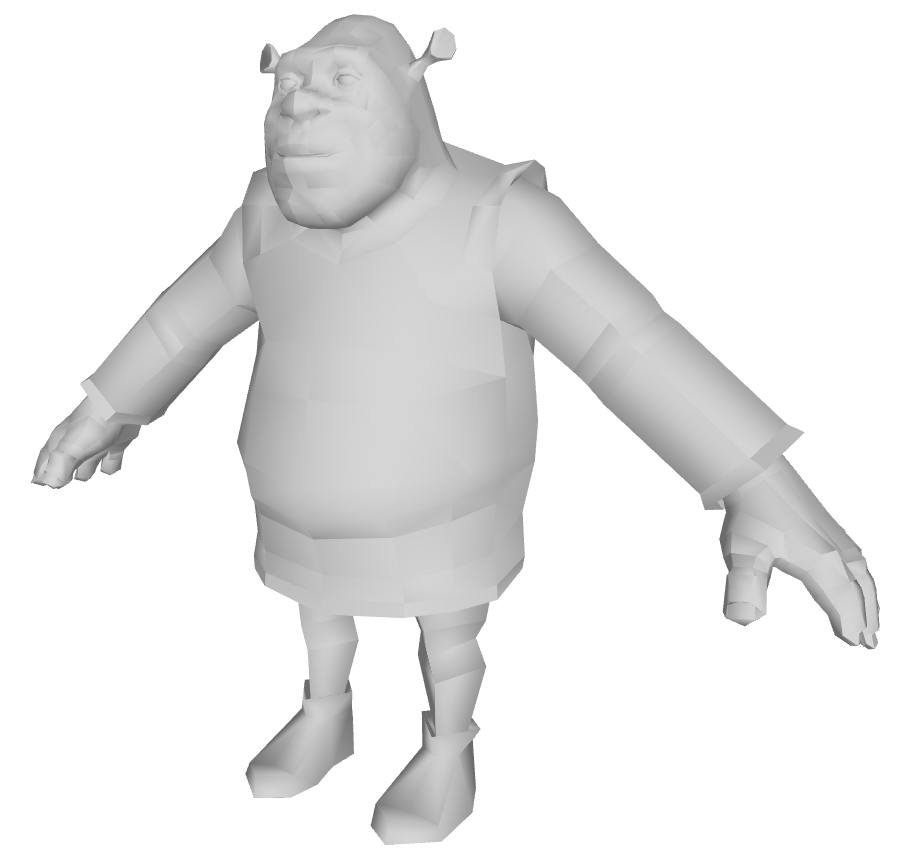
\includegraphics[width=\textwidth]{shrek.png}
        \caption {Testni model: Shrek}
        \label{model:shrek}
    \end{minipage}
    \begin{minipage}[b]{0.4\textwidth}
        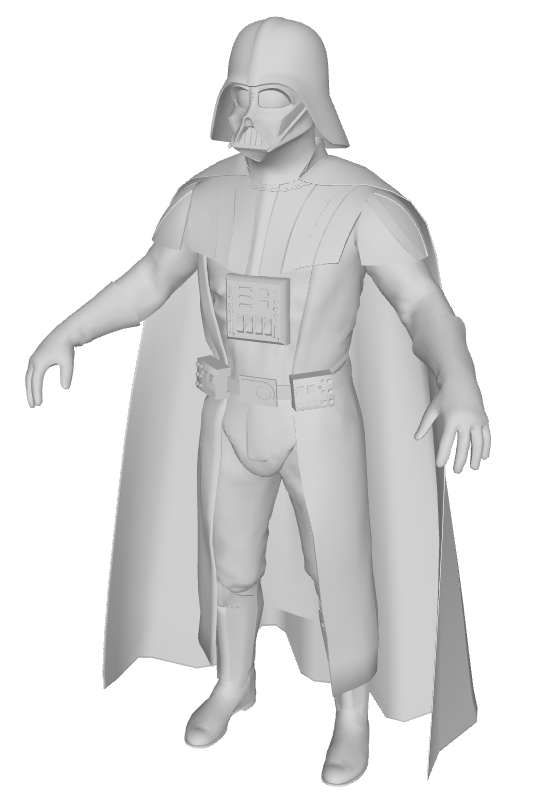
\includegraphics[width=\textwidth]{darthvader.png}
        \caption {Testni model: Darth Vader}
        \label{model:darthvader}
    \end{minipage}
\end{figure}

\begin{table}[h!]
    \begin{center}
      \begin{tabular}{ | c | c | c | c | }
        \hline
        \textbf{Modeli} & \textbf{Odnos objekata} & \textbf{Algoritam} & \textbf{Trajanje (ms)} \\
        \hline
         Cybertruck / Darth Vader & Sijeku se & Oktalno stablo & 68 \\
        \hline
         Cybertruck / Darth Vader & Sijeku se & Prostorno hashiranje & 82 \\
        \hline
         Cybertruck / Darth Vader & Sijeku se & Bruteforce & 643 \\
        \hline
         Shrek / Spiderman & Sijeku se & Oktalno stablo & 78 \\
        \hline
         Shrek / Spiderman & Sijeku se & Prostorno hashiranje & 517 \\
        \hline
         Shrek / Spiderman & Sijeku se & Bruteforce & 27839 \\
        \hline

         Cybertruck / Darth Vader & Ne sijeku se & Oktalno stablo & $<$1 \\
        \hline
         Cybertruck / Darth Vader & Ne sijeku se & Prostorno hashiranje & 10736 \\
        \hline
         Cybertruck / Darth Vader & Ne sijeku se & Bruteforce & 393867 \\
        \hline
         Shrek / Spiderman & Ne sijeku se & Oktalno stablo & $<$1 \\
        \hline
         Shrek / Spiderman & Ne sijeku se & Prostorno hashiranje & 685 \\
        \hline
         Shrek / Spiderman & Ne sijeku se & Bruteforce & 61512 \\
        \hline

         Cybertruck / Darth Vader & Sijeku se AABB-ovi & Oktalno stablo & 135 \\
        \hline
         Cybertruck / Darth Vader & Sijeku se AABB-ovi & Prostorno hashiranje & 4942 \\
        \hline
         Cybertruck / Darth Vader & Sijeku se AABB-ovi & Bruteforce & 394121 \\
        \hline
         Shrek / Spiderman & Sijeku se AABB-ovi & Oktalno stablo & 49 \\
        \hline
         Shrek / Spiderman & Sijeku se AABB-ovi & Prostorno hashiranje & 735 \\
        \hline
         Shrek / Spiderman & Sijeku se AABB-ovi & Bruteforce & 61512 \\
        \hline
      \end{tabular}
    \end{center}
  \caption{Rezultati testiranja}
  \label{table:testresults}
\end{table}
